\CQUsection{模型设计}

\CQUsubsection{研究方法总体框架}
本文面向颅内动脉瘤智能分析任务，构建了由病灶分割与破裂风险评估组成的两阶段研究框架。该框架遵循“病灶定位—结构表征—风险判别”的基本逻辑：首先利用三维分割网络对 CTA 体数据中的疑似动脉瘤区域进行体素级识别，获得病灶概率分布与空间掩膜；随后基于分割结果与病例层面的临床、形态及影像表型信息构建统一的特征表示，并输入风险预测模型完成患者级破裂概率估计。该流程兼顾了医学影像任务中局部解剖结构刻画与整体临床决策建模的双重需求。

从形式化角度看，设单例 CTA 体数据记为 $X\in\mathbb{R}^{D\times H\times W}$，其对应分割标注为 $Y^{(s)}\in\{0,1\}^{D\times H\times W}$，病例级风险标签为 $y^{(r)}\in\{0,1\}$。本文方法可表示为
\begin{align}
P &= f_{\theta}(X),\\
\hat{M} &= \mathcal{T}(P;\tau_s),\\
z &= \phi(X,\hat{M},c),\\
\hat{p} &= g_{\omega}(z),
\end{align}
其中，$f_{\theta}(\cdot)$ 表示分割网络，$P\in[0,1]^{D\times H\times W}$ 为体素级概率图，$\mathcal{T}(\cdot)$ 为基于阈值 $\tau_s$ 的二值化映射，$c$ 表示病例层面的临床及影像表型变量，$\phi(\cdot)$ 表示多源特征构造过程，$g_{\omega}(\cdot)$ 为风险预测模型，$\hat{p}\in[0,1]$ 为动脉瘤破裂概率估计。由此，本文实际上将像素级结构识别与样本级风险判别纳入统一分析链条，在保证解剖定位能力的同时增强风险建模的结构依据。

\CQUsubsection{分割任务的理论基础与建模动机}
颅内动脉瘤在 CTA 图像中通常表现为体积较小、边界复杂、与邻近血管结构相互黏连的异常膨出区域，因此分割任务具有显著的小目标、强背景干扰与类别不平衡特征。在此类场景下，单纯依赖局部卷积感受野容易产生两类问题：其一，浅层特征虽然保留空间细节，但缺乏足够语义判别能力；其二，深层特征具有较强抽象表示能力，却可能在多次下采样后损失病灶边界信息。U-Net 类结构通过编码器—解码器及跳跃连接机制较好地协调了上述矛盾，因此适合作为三维医学图像分割的基础框架。

然而，标准 U-Net 在复杂血管背景中仍可能引入大量与病灶识别无关的高响应区域。为此，本文在主干结构中引入注意力门控机制，以抑制无关背景特征在跳跃连接中的传播；同时在瓶颈层引入多尺度上下文增强与方向敏感注意力建模，以提升模型对病灶尺度变化、形态不规则性及空间走向复杂性的表达能力。该设计的理论动机在于：病灶分割并非仅依赖局部灰度差异，而是依赖于局部边界、邻域血管拓扑及多尺度上下文之间的联合判别。

\CQUsubsection{动脉瘤分割模块设计}
\CQUsubsubsection{输入表示与数据采样机制}
由于 CTA 体数据具有高维、稀疏和病例间差异较大的特点，本文首先对输入体数据进行统一空间归一化与强度规范化，以减弱扫描条件、体素间距与成像范围差异对模型学习带来的干扰。对于归一化后的三维影像，训练阶段采用基于局部补丁的学习方式，以在有限显存约束下维持足够的空间上下文范围；验证与测试阶段则通过覆盖式滑窗实现整例推理，保证输出结果的完整性与连续性。

考虑到动脉瘤区域在整幅体积中的占比通常远低于背景，若采用完全均匀采样策略，模型在训练过程中容易受到背景主导，进而导致前景召回不足。为此，本文采用兼顾前景强化与背景约束的补丁采样机制，即在训练样本构造时适当提高病灶邻域补丁的出现概率，以增强网络对少数类模式的感知能力，同时保留一定比例的背景补丁以维持正常解剖结构判别边界。该策略本质上是一种面向类别不平衡场景的数据分布重加权方法，有助于提高模型对小体积病灶的学习效率。

\CQUsubsubsection{三维 Attention U-Net 主干结构}
分割主干采用三维 Attention U-Net。编码器由多层三维卷积块和逐级下采样操作构成，用于提取从低层纹理到高层语义的分层特征；解码器则通过上采样和特征融合逐步恢复空间分辨率，实现精细的体素级预测。设第 $l$ 层编码器特征为 $E_l$，解码器特征为 $D_l$，则主干网络可抽象为
\begin{align}
E_l &= \mathcal{E}_l(E_{l-1}), \quad l=1,2,\ldots,L,\\
B &= \mathcal{B}(E_L),\\
D_l &= \mathcal{D}_l(D_{l+1},\widetilde{E}_l), \quad l=L-1,\ldots,1,
\end{align}
其中，$\mathcal{E}_l(\cdot)$ 表示第 $l$ 层编码映射，$\mathcal{B}(\cdot)$ 表示瓶颈层特征变换，$\mathcal{D}_l(\cdot)$ 表示第 $l$ 层解码映射，$\widetilde{E}_l$ 为经注意力筛选后的跳跃连接特征。通过这种由粗到细的层级重建过程，网络能够同时利用深层全局语义信息与浅层边界细节信息，从而提高病灶轮廓恢复能力。

\begin{figure}[htbp]
    \centering
    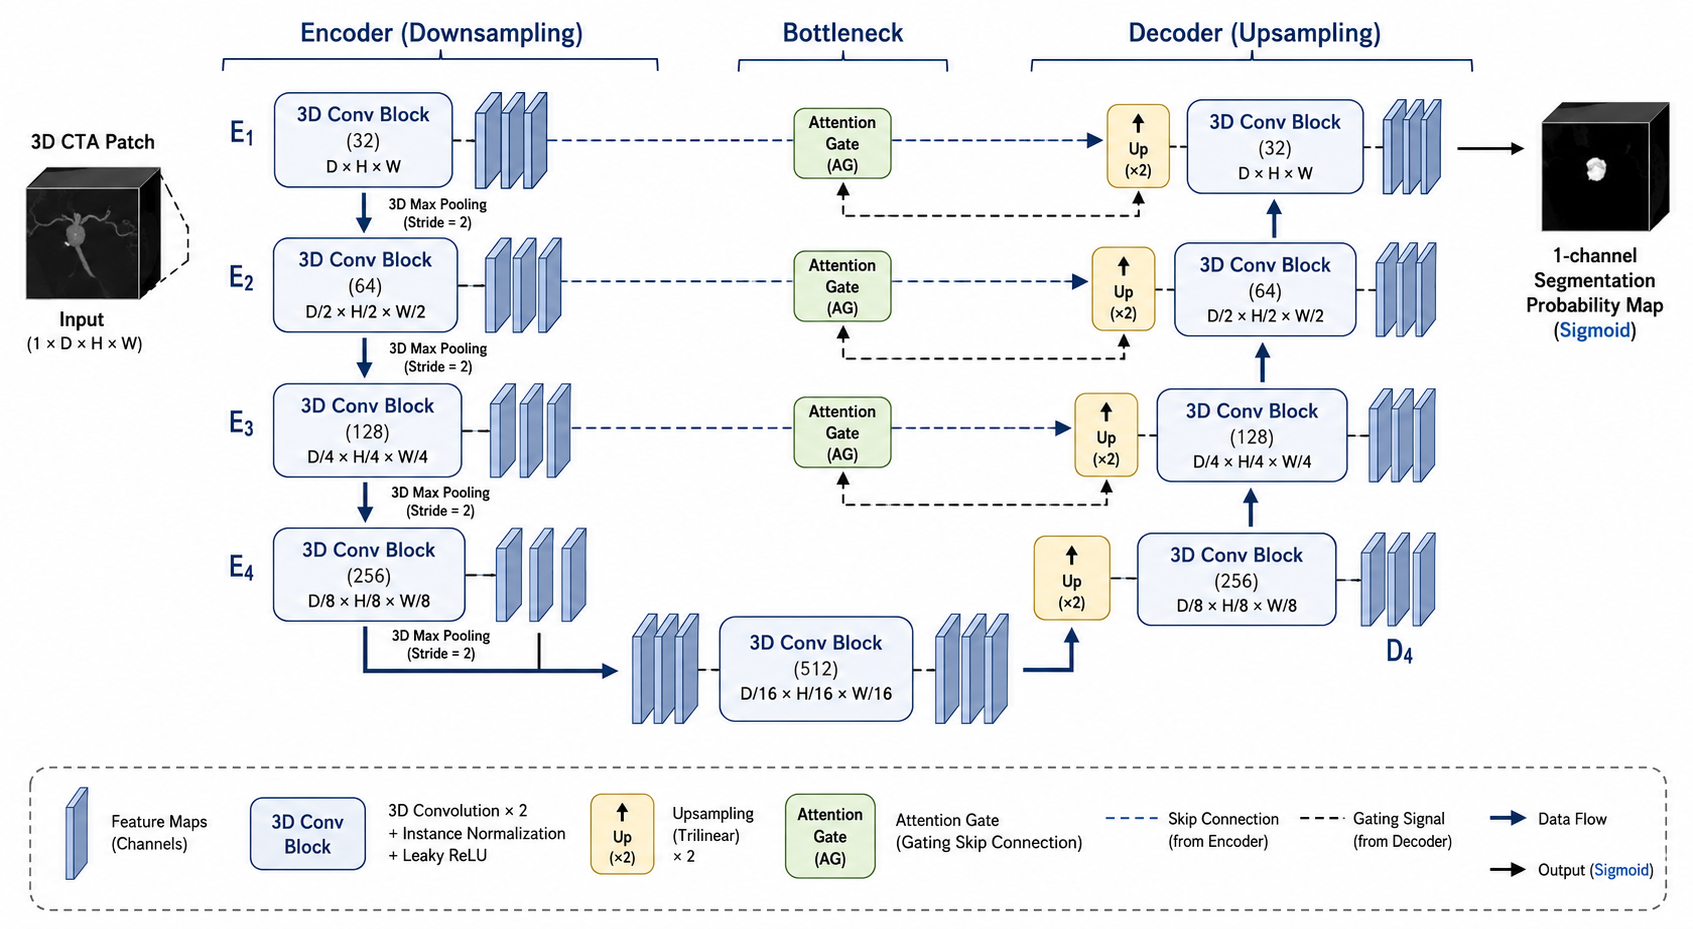
\includegraphics[width=0.95\textwidth]{figure/split_arch.png}
    \caption{三维 Attention U-Net 分割模型结构}
    \label{fig:split_arch}
\end{figure}

\CQUsubsubsection{注意力门控跳跃连接机制}
在传统 U-Net 中，编码器特征通常直接与对应尺度的解码器特征拼接。这种做法虽然有助于恢复空间分辨率，但也可能将大量背景响应一并引入解码过程，尤其是在血管、骨性结构及噪声干扰较强的 CTA 场景下更为明显。为缓解这一问题，本文在跳跃连接中采用注意力门控机制，使网络能够依据当前解码语义状态自适应选择更具判别力的编码特征。

设同尺度跳跃特征为 $s$，来自解码端的门控信号为 $g$，则注意力门控可写为
\begin{align}
q &= \mathrm{ReLU}(W_s s + W_g g + b),\\
a &= \sigma(\psi(q)),\\
\hat{s} &= a \odot s,
\end{align}
其中，$W_s$ 与 $W_g$ 为线性投影，$\psi(\cdot)$ 为通道压缩映射，$\sigma(\cdot)$ 为 Sigmoid 函数，$a$ 为取值于 $[0,1]$ 的注意力权重图，$\odot$ 表示逐元素乘法。该结构的本质是在跳跃连接处引入条件选择机制：当某些空间位置与当前解码语义更加一致时，对应权重被放大；反之，则被抑制。由此可降低无关背景特征对后续重建的干扰，提高分割结果的病灶聚焦能力。

\CQUsubsubsection{ASPP 多尺度上下文增强模块}
动脉瘤的空间形态在不同病例之间可能表现出明显差异，既包括局部球囊样膨出，也包括与载瘤血管边界过渡不清的复杂结构。因此，仅依赖固定尺度卷积核难以充分描述病灶及其邻近血管的多尺度上下文关系。为增强瓶颈层对不同尺度模式的响应能力，本文引入三维 ASPP 模块，通过多分支空洞卷积并行提取不同感受野下的上下文特征。

设瓶颈输入特征为 $X_b$，空洞率集合为 $\{d_1,d_2,\ldots,d_K\}$，则 ASPP 输出可表示为
\begin{equation}
Y_{\mathrm{ASPP}} = \phi\Bigl(\operatorname{Concat}\bigl[\mathcal{F}_{d_1}(X_b),\mathcal{F}_{d_2}(X_b),\ldots,\mathcal{F}_{d_K}(X_b)\bigr]\Bigr),
\end{equation}
其中，$\mathcal{F}_{d_k}(\cdot)$ 表示膨胀率为 $d_k$ 的三维空洞卷积分支，$\operatorname{Concat}[\cdot]$ 表示通道维拼接，$\phi(\cdot)$ 表示后续的线性融合与非线性映射。通过在同一层级聚合不同感受野的信息，模型能够更有效地刻画病灶本体、载瘤血管及局部背景之间的关系，从而增强对复杂形态病灶的识别鲁棒性。

\CQUsubsubsection{三维坐标注意力模块}
在多尺度上下文建模基础上，本文进一步引入三维坐标注意力模块，以增强网络对方向性位置信息的编码能力。与仅基于通道重加权的注意力形式不同，坐标注意力通过沿不同空间轴汇聚上下文信息，在保留位置依赖关系的同时生成方向敏感权重，因此更适合描述血管结构细长、走向复杂的空间特征。

设输入特征为 $X\in\mathbb{R}^{C\times D\times H\times W}$，则沿深度、高度与宽度方向的上下文聚合可分别表示为
\begin{equation}
Z_d=\operatorname{AvgPool}_{H,W}(X),\quad
Z_h=\operatorname{AvgPool}_{D,W}(X),\quad
Z_w=\operatorname{AvgPool}_{D,H}(X).
\end{equation}
三路聚合特征经共享映射与分支解码后得到三个方向注意力图 $A_d$、$A_h$ 与 $A_w$，最终输出为
\begin{equation}
Y_{\mathrm{CA}} = X \odot A_d \odot A_h \odot A_w.
\end{equation}
该模块通过显式建模空间方向依赖关系，使网络能够在保留通道语义的同时强化对关键位置的响应，有利于提升小病灶边界及空间走向敏感结构的识别精度。

\begin{figure}[htbp]
    \centering
    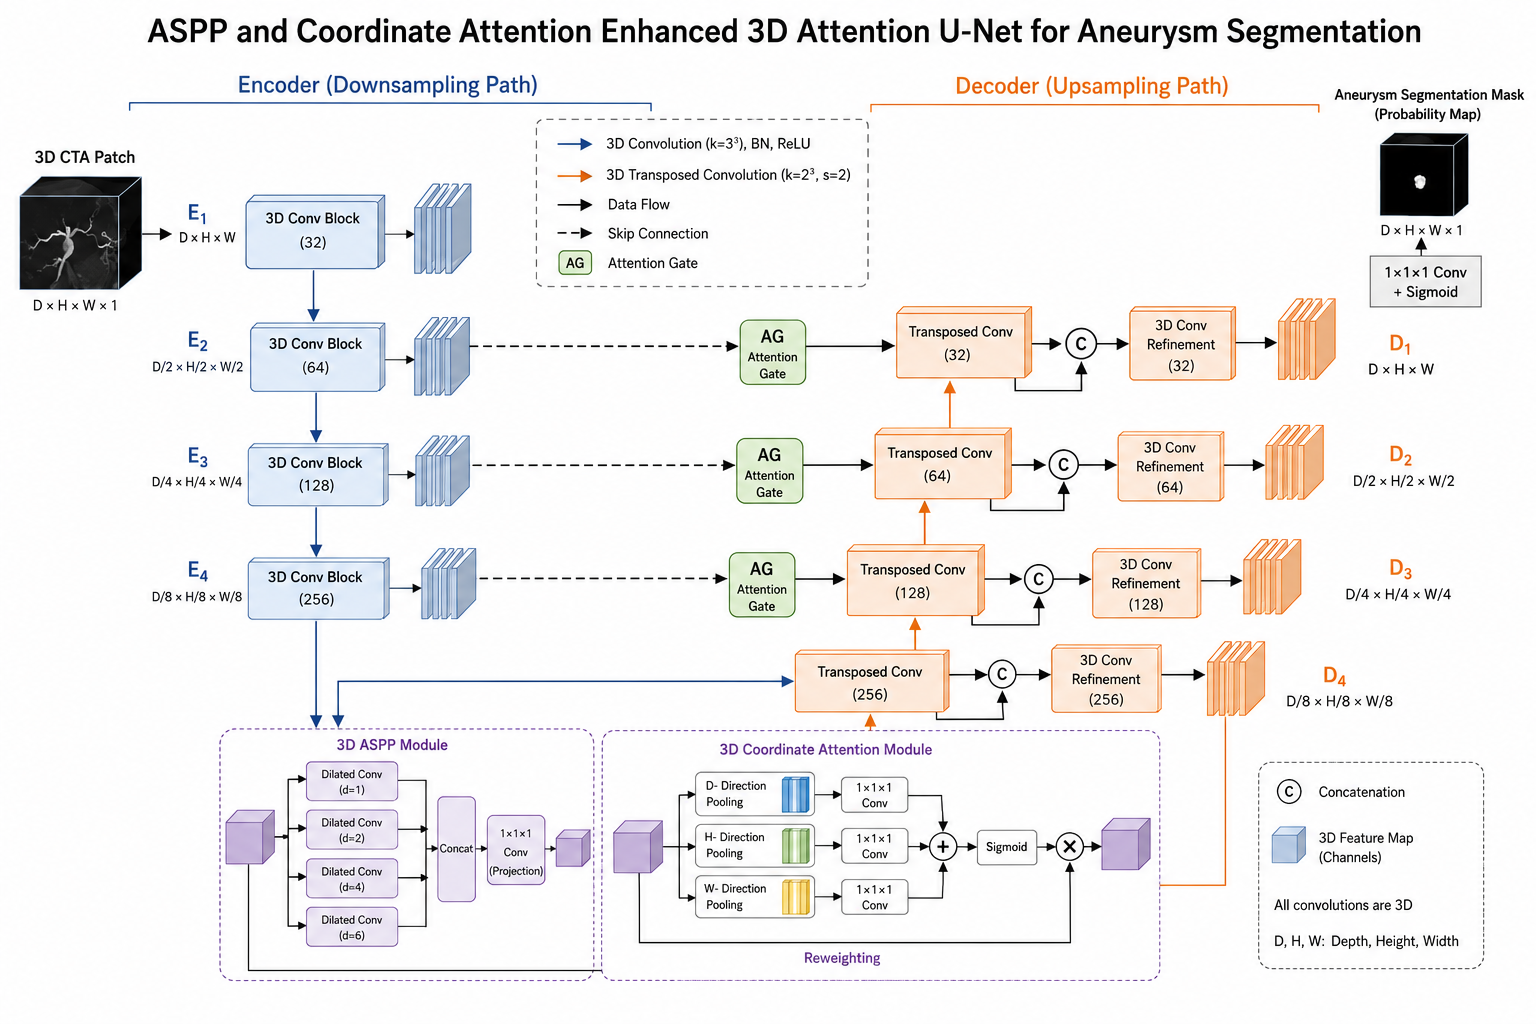
\includegraphics[width=0.95\textwidth]{figure/opt_split_arch.png}
    \caption{融合 ASPP 与三维坐标注意力的增强分割模型结构}
    \label{fig:opt_split_arch}
\end{figure}

\CQUsubsubsection{输出映射与整例重建}
在解码器末端，网络通过 $1\times1\times1$ 卷积将高分辨率特征映射到单通道对数几率空间，并经 Sigmoid 函数获得体素级前景概率图：
\begin{equation}
P_{i,j,k}=\sigma\bigl(h_{i,j,k}\bigr),
\end{equation}
其中，$h_{i,j,k}$ 表示位置 $(i,j,k)$ 处的输出 logit，$P_{i,j,k}$ 表示对应体素属于动脉瘤前景的概率。基于给定阈值 $\tau_s$，可得到二值掩膜
\begin{equation}
\hat{M}_{i,j,k}=\mathbb{I}(P_{i,j,k}\geq \tau_s),
\end{equation}
其中，$\mathbb{I}(\cdot)$ 为示性函数。

在整例推理阶段，由于输入体积较大，本文采用滑窗方式对局部补丁逐块预测，并将各窗口输出重新映射回原空间。对于重叠区域，可通过平均融合或中心区域优先策略进行整合，以减弱窗口边界效应。由此获得的整例概率图与二值分割结果，不仅可用于病灶可视化，也可进一步提取体积、尺寸及形态相关表型，为风险预测阶段提供结构性输入依据。

\CQUsubsubsection{分割损失函数与优化目标}
考虑到动脉瘤分割具有显著的前景稀疏特征，单独使用逐体素交叉熵损失容易使模型偏向背景预测，导致小病灶召回不足。为兼顾像素级分类准确性与区域重叠一致性，本文采用由二元交叉熵损失与重叠型损失组成的联合目标函数。

二元交叉熵损失定义为
\begin{equation}
\mathcal{L}_{\mathrm{BCE}} = -\frac{1}{N}\sum_{n=1}^{N}\left[y_n\log p_n + (1-y_n)\log(1-p_n)\right],
\end{equation}
其中，$N$ 为体素总数，$y_n\in\{0,1\}$ 为第 $n$ 个体素的真实标签，$p_n\in[0,1]$ 为对应预测概率。为进一步提高模型对前景区域及漏检错误的敏感性，本文引入 Tversky 型损失。设真阳性、假阳性和假阴性分别记为 $\mathrm{TP}$、$\mathrm{FP}$ 和 $\mathrm{FN}$，则 Tversky 系数可写为
\begin{equation}
\mathrm{TI} = \frac{\mathrm{TP}}{\mathrm{TP}+\alpha\,\mathrm{FP}+\beta\,\mathrm{FN}+\varepsilon},
\end{equation}
其中，$\alpha$ 与 $\beta$ 用于平衡假阳性与假阴性的惩罚权重，$\varepsilon$ 为避免分母为零的平滑项。对应损失可定义为
\begin{equation}
\mathcal{L}_{\mathrm{T}} = 1-\mathrm{TI}.
\end{equation}
因此，分割阶段总体优化目标写为
\begin{equation}
\mathcal{L}_{\mathrm{seg}} = \lambda_1\mathcal{L}_{\mathrm{BCE}} + \lambda_2\mathcal{L}_{\mathrm{T}},
\end{equation}
其中，$\lambda_1$ 与 $\lambda_2$ 为权重系数。该联合目标在理论上同时约束局部判别误差与整体区域重叠关系，适合小目标医学图像分割场景。

在优化过程中，模型参数通过基于梯度下降的自适应优化算法进行更新。设第 $t$ 次迭代的参数为 $\theta_t$，学习率为 $\eta_t$，则其更新形式可概括为
\begin{equation}
\theta_{t+1}=\theta_t-\eta_t\nabla_{\theta}\mathcal{L}_{\mathrm{seg}}(\theta_t).
\end{equation}
训练期间结合验证集性能对模型进行选择，从而在拟合能力与泛化能力之间取得平衡。

\CQUsubsection{破裂风险预测模块设计}
\CQUsubsubsection{多源特征表示与问题定义}
风险预测任务关注病例级破裂状态判别，与分割任务的体素级预测不同，其核心在于从多源异构变量中学习稳定的判别表示。设单个病例的输入由数值特征集合 $x^{(n)}\in\mathbb{R}^{m}$ 与类别特征集合 $x^{(c)}\in\mathbb{N}^{q}$ 构成，其中数值特征可包括临床指标、形态学统计量及影像表型描述，类别特征则对应离散化的病例属性。本文通过统一的数据清洗、缺失值处理与标准化策略将不同来源变量映射到可学习特征空间，并将问题定义为概率形式的二分类任务：
\begin{equation}
\hat{p}=\Pr(y^{(r)}=1\mid x^{(n)},x^{(c)}).
\end{equation}

与传统基于手工规则或浅层线性模型的方法相比，本文更关注变量之间潜在的非线性交互作用。例如，某一形态学指标对风险的影响可能依赖于年龄、病灶位置或其他影像表型变量，因此简单线性叠加往往难以充分表达这类高阶关联。为此，本文采用基于 token 表示与交叉注意力机制的表格深度模型，对异构字段之间的依赖关系进行显式建模。

\CQUsubsubsection{字段嵌入与统一隐空间映射}
为使数值特征与类别特征能够在同一模型中进行交互，需先将其映射到维度一致的隐空间。对于第 $i$ 个数值特征 $x_i^{(n)}$，本文通过可学习线性变换获得其嵌入表示：
\begin{equation}
e_i^{(n)} = W_i^{(n)} x_i^{(n)} + b_i^{(n)}, \quad i=1,2,\ldots,m,
\end{equation}
其中，$W_i^{(n)}$ 与 $b_i^{(n)}$ 为可学习参数。对于第 $j$ 个类别特征 $x_j^{(c)}$，其嵌入表示由查表方式获得：
\begin{equation}
e_j^{(c)} = \operatorname{Emb}_j\bigl(x_j^{(c)}\bigr), \quad j=1,2,\ldots,q.
\end{equation}
由此，所有字段均被表示为同维度向量，并共同组成字段级 token 序列
\begin{equation}
E = [e_1,e_2,\ldots,e_{m+q}]\in\mathbb{R}^{(m+q)\times d},
\end{equation}
其中，$d$ 为隐空间维度。该表示方式使模型能够将每个字段视为独立信息单元，从而为后续的注意力交互建模提供基础。

\CQUsubsubsection{交叉注意力特征交互机制}
本文风险模型的核心思想并非将全部字段直接拼接后输入分类器，而是通过注意力机制自适应学习字段间的相关性权重。设输入 token 表示为 $E$，经过线性映射得到查询、键和值矩阵：
\begin{equation}
Q=EW_Q,\quad K=EW_K,\quad V=EW_V,
\end{equation}
其中，$W_Q$、$W_K$ 与 $W_V$ 为可学习参数。字段间的相关性通过缩放点积注意力计算：
\begin{equation}
\operatorname{Att}(Q,K,V)=\operatorname{Softmax}\left(\frac{QK^{\top}}{\sqrt{d}}\right)V.
\end{equation}
对于多头注意力机制，可将上述过程扩展为多个子空间并行学习，再通过拼接与线性变换进行融合，从而提高对多类型交互关系的表达能力。

若进一步区分数值字段流与类别字段流，则交叉注意力可以刻画一类字段对另一类字段的条件依赖。例如，设数值字段表示为 $E^{(n)}$，类别字段表示为 $E^{(c)}$，则一种典型的跨模态交互形式可写为
\begin{equation}
\widetilde{E}^{(n)} = \operatorname{Att}\bigl(E^{(n)}W_Q^{(n)},E^{(c)}W_K^{(c)},E^{(c)}W_V^{(c)}\bigr),
\end{equation}
其含义是使用数值字段作为查询，以类别字段提供键和值，从而实现基于类别上下文的数值特征重表征。反向地，也可以构建由类别字段查询数值字段的交互通路。通过交替或叠加这两类交互映射，模型得以学习异构字段之间的双向依赖关系，从而形成更具判别力的病例级表示。

\CQUsubsubsection{全局聚合与风险概率输出}
在完成字段级交互后，模型需要将多 token 表示汇聚为病例级全局表征。设交互后的字段表示为 $H=[h_1,h_2,\ldots,h_{m+q}]$，则可采用平均池化、注意力池化或引入全局 token 的方式获得聚合向量 $r$：
\begin{equation}
r = \operatorname{Pool}(H).
\end{equation}
随后通过多层感知机完成最终判别，输出破裂风险概率：
\begin{equation}
\hat{p}=\sigma(W_o r + b_o).
\end{equation}
当给定分类阈值 $\tau_r$ 时，可得到病例级决策结果
\begin{equation}
\hat{y}^{(r)}=
\begin{cases}
1, & \hat{p}\geq \tau_r,\\
0, & \hat{p}<\tau_r.
\end{cases}
\end{equation}
这一过程使模型能够从字段级局部交互过渡到病例级整体判断，符合临床风险评估中“多因素综合判别”的基本思想。

\CQUsubsubsection{风险预测损失函数与类别不平衡处理}
破裂风险预测同样面临类别不平衡问题，即阳性样本数量通常少于阴性样本。若直接采用未加权的标准二元交叉熵，模型可能倾向于优先优化多数类准确率，从而削弱对少数类破裂病例的识别能力。为此，本文采用类别加权的二元交叉熵作为训练目标：
\begin{equation}
\mathcal{L}_{\mathrm{risk}} = -\frac{1}{N}\sum_{i=1}^{N}\left[w_1 y_i\log \hat{p}_i + w_0(1-y_i)\log(1-\hat{p}_i)\right],
\end{equation}
其中，$N$ 为样本数，$y_i$ 为第 $i$ 个病例的真实标签，$\hat{p}_i$ 为预测破裂概率，$w_1$ 与 $w_0$ 分别为阳性类与阴性类权重。通过增大少数类样本在损失函数中的贡献，可在一定程度上改善模型对高风险病例的敏感性。

在训练完成后，本文不直接固定使用 $0.5$ 作为分类阈值，而是基于验证集概率输出搜索最优阈值 $\tau_r^{\ast}$，使综合评价指标达到较优水平：
\begin{equation}
\tau_r^{\ast}=\arg\max_{\tau\in[0,1]}\mathcal{J}(\tau),
\end{equation}
其中，$\mathcal{J}(\tau)$ 可选取 F1 值、Youden 指数或其他适用于不平衡分类的综合准则。该策略有助于根据实际数据分布确定更合理的决策边界，提高风险预测的应用适配性。

\CQUsubsection{训练与优化过程}
本文整体训练过程遵循监督学习范式。对于分割任务，网络通过最小化体素级联合损失学习从三维影像到病灶概率图的映射；对于风险预测任务，模型通过最小化加权分类损失学习从病例级特征表示到破裂概率的映射。两个任务分别在训练集上进行参数更新，在验证集上完成模型选择与超参数调节，并在独立测试集上报告最终性能。

从优化角度看，训练过程本质上是在参数空间中求解经验风险最小化问题：
\begin{equation}
\theta^{\ast}=\arg\min_{\theta}\frac{1}{N}\sum_{i=1}^{N}\mathcal{L}(x_i,y_i;\theta),
\end{equation}
其中，$\mathcal{L}(\cdot)$ 对于不同任务分别对应 $\mathcal{L}_{\mathrm{seg}}$ 与 $\mathcal{L}_{\mathrm{risk}}$。为提高训练稳定性，优化过程中结合学习率调度、验证监控及最优检查点保留策略，以降低随机波动对最终结果的影响。该过程既保证了模型能够充分拟合训练分布，又为后续实验比较提供了统一且可复核的评价基础。

\CQUsubsection{本章小结}
本章系统阐述了本文所采用的研究方法与模型设计。首先，从整体框架层面明确了“分割先验驱动风险评估”的两阶段分析思路；其次，围绕三维 Attention U-Net、注意力门控、ASPP 与三维坐标注意力等关键模块，对动脉瘤分割模型的结构组成、输入输出关系与优化目标进行了理论化描述；再次，对风险预测模型中的字段嵌入、交叉注意力交互、全局聚合、加权损失及阈值搜索策略进行了形式化说明。总体而言，本文方法通过多尺度空间表征与多源特征融合相结合，为后续实验验证与结果分析奠定了方法学基础。